\documentclass{article}

\usepackage[a4paper, total={6in, 8in}]{geometry}

\usepackage{amsmath}
\usepackage{amsfonts}
\usepackage{amssymb}
\usepackage[T1, T2A]{fontenc}
\usepackage[utf8]{inputenc}
\usepackage[english, russian]{babel}
\usepackage{graphics}
\usepackage{graphicx}

\geometry{
 a4paper,
 total={170mm,257mm},
 left=20mm,
 top=20mm,
 }

\author{Александр Валентинов}
\title{Лабораторная работа 3.6.1}

\begin{document}
   \subsection*{Работа 3.2.6}
   \section*{Исследование гальванометра}
   
   \paragraph{Цель работы:} изучение работы высокочувствительного зеркального гальванометра магнитоэлектрической системы в режимах измерения постоянного тока и электрического заряда.
   
   \paragraph{В работе используются:} зеркальный гальванометр с осветителем и шкалой, источник постоянного напряжения, делитель напряжения, магазин сопротивлений, эталонный конденсатор, вольтметр, преключатель, ключи, линейка.

   \subsubsection*{Установка.}
   \begin{figure}[h]
   \centering
   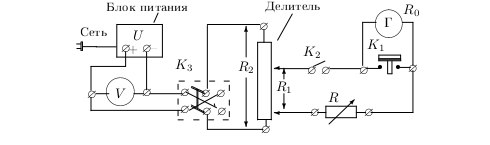
\includegraphics[width=10cm]{fig1.jpg} 
   \caption{Схема установки для работы гальванометра в стационарном режиме.} 
   \label{fig.1} 
   \end{figure}

   \begin{figure}[h]
   \centering
   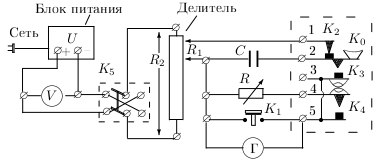
\includegraphics[width=7cm]{fig2.jpg} 
   \caption{Схема установки для определения баллистической постоянной.} 
   \label{fig.2} 
   \end{figure}

   \subsubsection*{Теория.}
   Сила тока, протекающего через гальванометр в стационарном режиме:
   \begin{equation}
   \label{fl.1}
   I = U_0 \frac{R_1}{R_2}\frac{1}{R + R_0}.
   \end{equation}
   Динамическая постоянная:
   \begin{equation}
   \label{fl.2}
   C_I = \frac{I}{\varphi} = \frac{2aI}{x}, \quad \sigma_{C_I} = \sqrt{\left( \frac{I}{x}\sigma_{2a} \right)^2 + \left( 2a \sigma_{\frac{I}{x}} \right)^2}.
   \end{equation}
   Логарифмический декремент затухания:
   \begin{equation}
   \label{fl.3}
   \Theta = \ln \frac{x_n}{x_{n + 1}}, \quad \sigma_\Theta = \sqrt{\left(\frac{\sigma_{x_n}}{x_n}\right)^2 + \left( \frac{\sigma_{x_{n + 1}}}{x_{n + 1}} \right)^2}.
   \end{equation}
   Критическое сопротивление ($X = (R_0 + R)^2$, $Y = 1 / \Theta^2$):
   \begin{equation}
   \label{fl.4}
   R_{\text{кр}} = \frac{1}{2\pi}\sqrt{\frac{\Delta X}{\Delta Y}} - R_0, \quad \sigma_{R_\text{кр}} = \frac{1}{4\pi} \sqrt{\frac{\Delta Y}{\Delta X}} \cdot \sigma_{\frac{\Delta X}{\Delta Y}}.
   \end{equation}
   Баллистическая постоянная:
   \begin{equation}
   \label{fl.5}
   C_{Q_\text{кр}} = 2a \frac{R_1}{R_2} \frac{U_0 C}{l_{max}^\text{кр}}
   \end{equation}
   \subsubsection*{Обработка результатов.}
   Рассчитаем ток через гальванометр в стационарном режиме по формуле \eqref{fl.1}. Построим график $I(x)$ (таблица \ref{table1}, рисунок \ref{plot.1}. С его помощью найдем динамическую постоянную по формуле \eqref{fl.2}. Заметим, что погрешность измерения $R$ и $R_0$ пренебрежимо мала по сравнению с $x$.
   \[
      \frac{I}{x} = (22.8 \pm 0.5) \cdot 10^{-6} \text{ А}/\text{м}
   \]
   \[
      C_I = (0.0501 \pm 0.0016) \frac{\text{А}}{\text{ мм}/\text{м}}.
   \]

   \begin{table} 
 \caption{Зависимость для RC-цепи}
 \label{RCtable}
\begin{center}
\begin{tabular}{|*{4}{r|}}
\hline 
$\psi$ & $\tan \psi$ & $\sigma_{\tan_\psi}$ & $1 / (\Omega C R_\Sigma)$ \\ \hline 
 1.51 & 16   & 1    & 25.7  \\ \hline 
 1.26 & 3.1  & 0.2  & 2.83  \\ \hline 
 1.01 & 1.6  & 0.1  & 1.65  \\ \hline 
 0.75 & 0.94 & 0.09 & 0.93  \\ \hline 
 0.50 & 0.55 & 0.07 & 0.566 \\ \hline 
 0.25 & 0.26 & 0.07 & 0.260 \\ \hline 
 0.00 & 0.00 & 0.06 & 0.099 \\ \hline 
 \end{tabular}
\end{center} 
\end{table} 

   \begin{figure}[h]
   \centering
   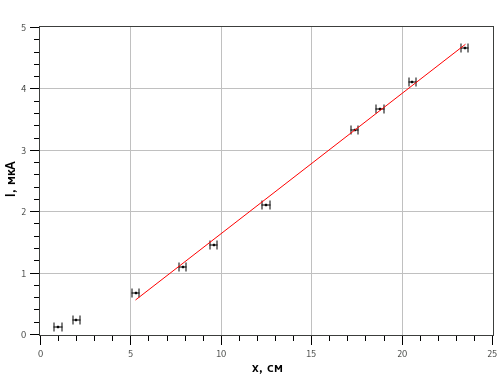
\includegraphics[width=12cm]{plot1.png} 
   \caption{Зависимость $I(x)$.} 
   \label{plot.1} 
   \end{figure}

   Рассчитаем логарифмический декремент затухания по формуле \eqref{fl.3}. Построим график $1/\Theta^2 = f\left[ (R + R_0)^2 \right]$ (таблица \ref{table2}, рисунок \ref{plot.2}). Рассчитаем погрешность $1 / \Theta^2$ по формуле
   \[
       \sigma_{1/\Theta^2} = \frac{\sigma_\Theta}{\Theta^3}.
   \]
   Погрешность $R$ и $R_0$ пренебрежимо мала. С помощью графика рассчитаем критическое сопротивление, пользуясь формулой \eqref{fl.4}.
   \[
      \frac{\Delta X}{\Delta Y} = 1 / \frac{\Delta Y}{\Delta X}, \quad \sigma_{\frac{\Delta X}{\Delta Y}} = \sigma_{\frac{\Delta Y}{\Delta X}} / \left(\frac{\Delta Y}{\Delta X}\right)^2.
   \]
   \[
      \frac{\Delta Y}{\Delta X} = (0.0194 \pm 0.0007) \text{ кОм}^{-2}
   \]
   \[
      R_{\text{кр}} = (860 \pm 30) \text{ Ом}
   \]

   \begin{table} 
 \caption{Table2}
\begin{tabular}{|*{8}{c|}}
\hline 
I & Ex0.3 & Ex0.45 & Ex0.5 & Ex0.65 & Ex0.8 & Ex0.95 & Ex-0.95\\ \hline 
17.2 & 0 & 0 & 0 & 0 & 0 & 0 & 0 \\ \hline 
 181.9 & 0.051 & 0.072 & 0.084 & 0.109 & 0.129 & 0.159 & 0.166 \\ \hline 
 378.1 & 0.103 & 0.151 & 0.169 & 0.218 & 0.266 & 0.319 & 0.328 \\ \hline 
 571.8 & 0.151 & 0.224 & 0.251 & 0.322 & 0.396 & 0.472 & 0.496 \\ \hline 
 730.7 & 0.195 & 0.288 & 0.323 & 0.417 & 0.508 & 0.605 & 0.64 \\ \hline 
 854.4 & 0.228 & 0.336 & 0.378 & 0.487 & 0.595 & 0.71 & 0.75 \\ \hline 
 934.9 & 0.251 & 0.368 & 0.418 & 0.535 & 0.655 & 0.781 & 0.831 \\ \hline 
 1,003 & 0.269 & 0.394 & 0.446 & 0.569 & 0.698 & 0.83 & 0.884 \\ \hline 
 \end{tabular} 
\end{table} 

   \begin{figure}[h]
   \centering
   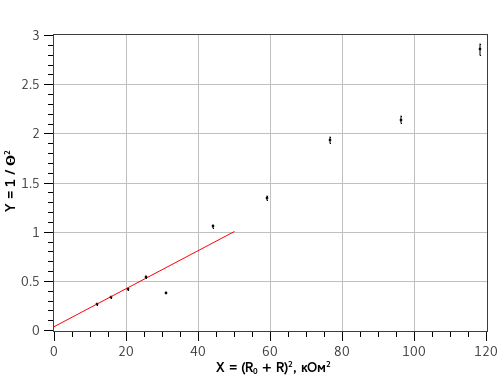
\includegraphics[width=12cm]{plot2.png} 
   \caption{Зависимость $1 / \Theta^2\left[ (R_0 + R)^2 \right]$.} 
   \label{plot.2} 
   \end{figure}

   Рассчитаем критическое сопротивление для баллистического режима. Для этого построим график $l_{max}\left[ (R + R_0)^{-1} \right]$ (таблица~\ref{table3}, рисунок~\ref{plot.3}), учтем, что отклонение зайчика в критическом режиме в $e$ раз меньше, чем в режиме без затухания. Отклонение в режиме без затухания $l_{max}^0 = (23.6  \pm 0.1)\text{ см}$, значит в критическом режиме $l_{max}^\text{кр} = (8.68 \pm 0.04)\text{ см}$. Коэффициент наклона графика $k = (-19.5 \pm 0.6)\text{ см}\cdot\text{кОм}$.
   \[
       R_\text{кр} = \frac{k}{l_{max}^\text{кр} - l_{max}^0} - R_0, 
   \] 
   \[
      R_\text{кр} = (1020 \pm 30) \text{ Ом}
   \]
   
   \begin{table} 
 \caption{Table3}
\begin{tabular}{|*{3}{c|}}
\hline 
f & delta nu & 1\\ \hline 
1 & 1.0 & 0.1 \\ \hline 
 2 & 2.0 & 0.2 \\ \hline 
 3 & 2.5 & 0.1 \\ \hline 
 4 & 5.0 & 0.5 \\ \hline 
 5 & 5.0 & 0.6 \\ \hline 
 6 & 5.7 & 0.5 \\ \hline 
 7 & 6.7 & 0.7 \\ \hline 
 8 & 7.5 & 0.8 \\ \hline 
 \end{tabular} 
\end{table} 

   \begin{figure}[h]
   \centering
   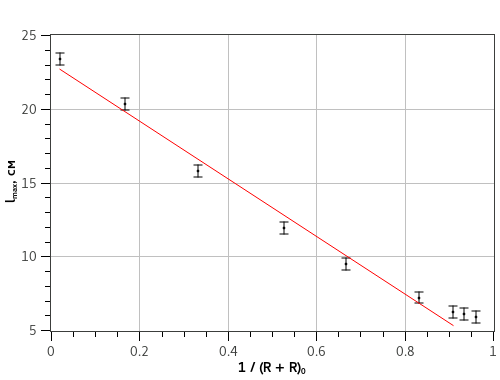
\includegraphics[width=12cm]{plot3.png} 
   \caption{Зависимость $l_{max}\left[ (R + R_0)^{-1} \right]$.} 
   \label{plot.3} 
   \end{figure}

   Значения, полученные подбором, в стационарном и баллистическом режиме совпадают.

   Рассчитаем баллистическую постоянную по формуле \eqref{fl.5}:
   \[
      C_{Q_\text{кр}} = (0.0100 \pm 0.0003) \frac{\text{К}}{\text{мм} / \text{м}}.
   \]

   Время релаксации $ t = R_0 C = 560 \text{ мкс} \ll T = 5 \text{ с}$
\end{document}
